\documentclass[twoside]{article}
\usepackage{amssymb}
\usepackage{amsmath}
\usepackage{algorithm}
\usepackage{algpseudocode}
\usepackage{pgfplots}
\usepackage{multicol}
\usepackage[hmarginratio=1:1,top=32mm,columnsep=20pt]{geometry}
\usepackage{fullpage}
\usepackage{pdflscape}
\usepackage{tikz}
\usepackage[toc,page]{appendix}
\usepackage[shortlabels]{enumitem}\usepackage{draftwatermark}

\newcommand{\quotes}[1]{``#1''}

\begin{document}
\parindent=0in
\parskip=12pt

\SetWatermarkText{Draft}
\SetWatermarkScale{5}

\title{
  Relative Probability on Finite Sample Spaces \\
  \large{
    SUBTITLE HERE
  }
}

\author{Max Sklar\\ Local Maximum Labs \\ DATE HERE}
\date{}

\maketitle
\thispagestyle{empty}

\begin{abstract}
This is an obviously incomplete draft/outline of an upcoming paper. Please do not share
\end{abstract}

\section{Introduction}

It may surprise many that the mathematical foundations of probability theory are still very much open to debate.

Since Kolmogorov published the standard axioms for probability theory in 1933, there have been calls to relax some of those assumptions and rules for various applications. In the paper Kolmogorov's Axiomatisation and Its Discontents\cite{lyon}, Lyon lays out these cases and their justification. One of difficult questions is the definition of a condiational probability where the condition has a probability of zero. Informally, this means that we wish to talk about the probability of an event given a hypothetical situation which will not occur\footnote{There is another very unintuitive feature of probability theory zero probability events do indeed occur all the time, particularly when given a continuous distribution.}. Related to this question is whether we can talk about the relative probability of two events in a system, even though those two events may have probability zero.

The standard model defines these values as a ratio of one probability to another. As a result, every time the indeterminate form \(\frac{0}{0}\) appears, the relative probability must remain undefined. Undeterred by this state of affairs, mathematicians and engineers talk about this type of relative probability all the time. For example, if we consider the continuous probability distributrion over \([0, 1]\) given by the probability distribution function \(2x\), we know that the PDF at \(x = \frac{1}{2}\) is twice as much as the PDF at \(x = \frac{1}{4}\). In a sense, we believe that the former is twice as likely as the latter - even though we are only talking about \textit{probability density} or \textit{PDF} values.

Let us take the position that we may model probability in a non-standard way, and we can do so as long as the framework is logically consistent, and the advertised applications match such a proposal\footnote{Lyon identifies this link to application as the bridge principle. A new set of axioms for probability could well give rise to a new and interesting mathematics, but if that mathematics cannot be linked to any application that a person would reasonbly call probability, then it ought to go by a different name.}. Given the popularity of Bayesian methods as applied to machine learning in recent decades, and given that the methods used to search a hypothesis space in Bayesian inference relies on relative probability\cite{sklar_bias}, we ought to understand whether we can derive a framework for probability that takes the relationships between outcomes and events as fundamental.

Not only would this solve the conditional probability question, but it would also give rise to several new concepts and objects to study. In this paper we will construct a theory of relative probability on finite distributions as a starting point for more complexity in future work. As we shall see, even for this simple case there is much work to be done!

We will also look at potential applications of these ideas, including limit distributions, bayesian inference, and even implementation.

These methods have applications in Bayesian statistics, even providing a new formulation of Bayes rule. This new formulation is reflective of current practice.

\section{Preliminaries}
\subsection{Magnitude Space}

Let \(\mathbb{M} = [0, +\infty]\) be the space of \textit{magnitudes}, which roughly corresponds with our intuition for the concept of size. The magnitude space contains all positive real numbers, \(0\) and \(\infty\).

The following functions are defined for all \(m_1, m_2\) in \(\mathbb{M}\).

\(\mathbb{M}\) is closed under addition. \(m_1 + m_2\) is the sum of \(m_1\) and \(m_2\).

\[m + \infty = \infty\]

The products \(0 \cdot \infty\) and \(\infty \cdot 0\) are indeterminate. In all other cases, multiplication on \(\mathbb{M}\) is defined.

The multiplicative inverse \(m^{-1}\) is the defined on all \(\mathbb{M}\). We let \(0^{-1} := \infty\) and \(\infty^{-1} := 0\), even though it doesn't quite act as a multiplicative inverse in those cases.

Any magnitude can be raised to the power of a real number and still be a magnitude.

\(\forall x \in \mathbb{R}, m^x \in \mathbb{M}\).

If we consider the \textit{extended real number line} to contain values at \(+\infty\) and \(-\infty\), we can continue to define these exponential operations, except for when \(m = 1\):

If \(m > 1\), then \(m^{+\infty} = \infty\) and \(m^{-\infty} = 0\)
If \(m < 1\), then \(m^{+\infty} = 0\) and \(m^{-\infty} = \infty\)

The set of magnitudes is a totally ordered set under \(\leq\), meaning that for every two magnitudes either \(m_1 \leq m_2\) or \(m_2 \leq m_1\), and if both are true then \(m_1 = m_2\)

\subsection{The Wildcard Element}

\[\mathbb{M}^* = \mathbb{M} \cup \{\ast\}\]

Let the \textit{magnitude-wildcard space} \(\mathbb{M}^*\) be defined as the set of magnitudes along with a \textit{wildcard element}, \(\ast\). The wildcard element corresponds to several different ideas depending on the context:
\begin{itemize}
  \item The \textit{wildcard pattern} used in pattern matching and regular expressions in type theory and computer science
  \item The indeterminate form \(\frac{0}{0}\) in arithmatic.
  \item The standard \textit{NaN}, or \textit{Not a Number}\footnote{\quotes{Not a Number} may have been an unfortunate choice, because it might actually represent \textbf{any} number!} value in the IEEE standard for floating point arithmetic.
\end{itemize}

We define the following properties on \(\ast\):
\[0 \cdot \infty = \ast\]
\[\ast + m = \ast\]
\[\ast \cdot m = \ast\]

Let the \textbf{matching relation}\footnote{It helps to read \(:\cong\) as \quotes{is matched by}.} \(:\cong\) be a binary relation on \(\mathbb{M}^*\) with the following properties.

-----------------------

Property 1: Every element is matched by the wildcard element. \[m :\cong \ast\].
Property 2: The wildcard element is matched only by itself. \[\ast :\cong m \Longrightarrow m = \ast\].

Property 3: If an element is matched by a non-wildcard element, then it is equal to it. 
\[m_1 :\cong m_2 \text{and} m_2 \neq \ast \Longrightarrow m_1 = m_2\]


The matching relation is not symmetric. It is asking if the element on the left hand side could be represented by the element on the right hand side. The wildcard element represents every single value, but it cannot be said to be represented by any singular value. To put it another way, the wildcard element represents a loss of information about a value which can never be recovered.

Theorem: The matching relation is transitive. In other words, for all \(m_1, m_2, m_3\) in \(\mathbb{M}\), if \(m_1 :\cong m_2\) and \(m_2 :\cong m_3\), then \(m_1 :\cong m_3\).

Proof: Assume that \(m_1 :\cong m_2\) and \(m_2 :\cong m_3\). If none of these values are the wildcards, then by property 1 (cite in latex), they are all equal and \(m_1 :\cong m_3\). If \(m_1 = \ast\) then by proerty 3 (cite), \(m_2 = \ast\) and finally \(m_3 = \ast\) so the theorem holds. If \(m_2 = \ast\) then \(m_3 = \ast\) and \(m_1 :\cong m_3\) by property 2 (cite). And of course if \(m_3 = \ast\) alone, then by property 2 \(m_1\) is still matched by \(m_3\).

Theorem: The matching relation preserves multiplication.

\begin{equation}
\label{eq:matching_multiplication}
\forall a,b,a',b' \in \mathbb{M}, a :\cong a' \wedge b :\cong b' \Rightarrow ab :\cong a'b'
\end{equation}

\section{Categorical Distribution}

\subsection{Definition}

Let \(\Omega\) be a finite set of mutually exclusive \textit{outcomes}. Because we assume that \(\Omega\) is finite, we can count its members as \(|\Omega| = K\). We say there are \(K\) outcomes, or \textit{categories}.

A \textit{categorical distribution} on a \(\Omega\) is a function \(P: \Omega \rightarrow [0, 1]\) such that \(\sum_{h \in \Omega} P(h) = 1\)

The set of all categorical distributions can be embedded in \(\mathbb{R}^K\) as a (K-1)-dimentional object called a (K-1)-simplex. For example, if \(K = 3\), the resulting space of categorical distributions is an equilateral triangle embedded in \(\mathbb{R}^3\) connecting the points (1, 0, 0), (0, 1, 0), and (0, 0, 1).

Because the set of categorical distributions is embedded in Euclidean space \(\mathbb{R}^K\), it's properties are well understood. We take the topology of the simplex to be the sub-topology of \(\mathbb{R}^K\). The simplex is also closed, bounded, and compact. (DO WE NEED THIS DETAIL?)

\subsection{Events}

An \textit{event} is a set of outcomes. We define \(\mathcal{F}\) as the space of all possible events. \(\mathcal{F}\) is the power set\footnote{In general, \(\mathcal{F}\) is not the entire power set of \(\Omega\) but typically is when \(\Omega\) is finite.} of \(\Omega\), meaning that \(\mathcal{F} = \mathcal{P}(\Omega)\), and for any event \(e \in \mathcal{F}\), \(e \subseteq \Omega\).

In the previous section, we defined the probability of individual outcomes. We can now define the probability function on events instead of outcomes. For finite distributions, this is simple. For all \(e\) in \(\mathcal{F}\),
\[ P(e) = \sum_{h \in e}{P({h})}\]

We can take the function \(P\) as acting either on outcomes or events using the convention \(P(\{h\}) = P(h)\). 

That \(\Omega\) itself the \textit{universal event} of all outcomes with \(P(\Omega) = 1\).

TODO: Properties of events: union, intersection, etc [NEEDED?]

\subsection{Relative Probability Function}

The \textit{relative probability function}, or \textit{RPF}, measures the probability of one event with respect to another. In some cases, we might wish to talk about events that are, for example, \quotes{twice as likely}, even if we don't know the absolute probability of either event.

We continue to use P to represent the RPF but with 2 inputs instead of 1. The expression \(P(e_1, e_2)\) can be read as the probability of \(e_1\) relative to \(e_2\).

\[P: \mathcal{F} \times \mathcal{F} \rightarrow \mathbb{M}^*\]

We define relative probability in terms of absolute probability as follows.

\[P(e_1, e_2) = \frac{P(e_1)}{P(e_2)}\]

Theorem: \[\forall e_1, e_2, e_3 \in \mathcal{F}, P(e_1, e_3) :\cong P(e_1, e_2) \cdot P(e_2, e_3)\]

Proof: Start with the case that \(e_2 \neq 0\). Then \(P(e_1, e_2) \cdot P(e_2, e_3) = \frac{P(e_1)}{P(e_2)}\frac{P(e_2)}{P(e_3)} = \frac{P(e_1)}{P(e_3)} = P(e_1, e_3)\). When \(e_2 = 0\), \(P(e_1, e_2) \cdot P(e_2, e_3) = \frac{P(e_1)}{P(e_2)}\frac{P(e_2)}{P(e_3)} = \ast\). Because \(\ast\) matches everything, then the matching statement holds. Because it holds in both cases, the theorem is true.

\section{Relative Categorical Distribution}

In the last section, the relative probability function was derived from the absolute probability function. In this section, we start with the relative probability function as the fundamental object of study.

\subsection{Relative Probability Functions on Outcomes}

Consider a relative probability function \(P\) that acts on outcomes only.

\[P: \Omega \times \Omega \rightarrow \mathbb{M}^*\]

The expression \(P(h_1, h_2)\) can be read as the probability of \(h_1\) relative to \(h_2\). A relative probability function is valid if and only if it obeys \textit{the fundamental property of relative probability} as follows.

\begin{equation}
\label{eq:fundamental}
\forall h_1, h_2, h_3 \in \Omega, P(h_1, h_3) :\cong P(h_1, h_2) \cdot P(h_2, h_3)
\end{equation}

We also require that \(\forall h \in \Omega, P(h, h) = 1\) which can be proven by the fundamental property in most circumstances.

Our next task is to upgrade \(P\) to operate on the event level. The relative probability of two events is going to be the ratios of their absolute probabilities [REFER TO PREVIOUS EQUATION], but we no longer have access to absolute probability. So, the best we can do is measure relative probability to a given event \(h^*\). Because this ratio might be indeterminate, we use the matching relation instead of equality.

For all \(h^* \in \Omega\), \[P(e_1, e_2) :\cong \frac{\sum_{h_1 \in e_1} P(h_1, h^*)}{\sum_{h_2 \in e_2} P(h_2, h^*)}\]

While this is a true statement, does it work as a definition? An alternate definition could be \[P(e_1, e_2) = \sum_{h_1 \in e_1} \frac{1}{\sum_{h_2 \in e_2} p(h_2, h_1)}\], but it has an exception that for \(P(\{\},\{\}) = 1\). TODO: Come up with a better definition.

Theorem: The fundamental theorem on the event level.

We then derive the absolute probability function as

\[P(e) = \sum_{h \in e} \frac{1}{\sum_{h' \in \Omega}p(h', h)}\]

The reversed comparison theorem: For all RPF \(P\) and events \(e_1\) and \(e_2\), \(P(e_1, e_2) = P(e_2, e_1)^{-1}\).

Proof: FILL IN

\subsection{Degenerate Cases}

Suppose that \(K = 0\). This means that \(\Omega\) is empty, and there are no outcomes. Surprisingly, there is still an RPF because there is one outcome represented by the empty set \(\varnothing\). In this case \(P(\varnothing, \varnothing) = 1\) is the only RPF. This is a mathematical bybproduct of our definition, but an interesting comparison to the case of absolute distributions where such a function does not exist (because without outcomes, it cannot add to 1).

Consider the case where \(K = 1\), and \(\Omega = {h}\). There is still only a single, trivial RPF P, where \(P(h, h) = 1\), and \(P(\varnothing, h) = 0\). This matches the absolute case where the probability of the single outcome must be 1.

\subsection{Matching and Equality}

Let \(P_1\) and \(P_2\) be relative probability functions. Define the concept of \(P_1\) being matched by \(P_2\) as:

\(P_1 :\cong P_2\) if and only if \(\forall e_1, e_2 \in \mathcal{F}, P_1(e_1, e_2) :\cong P_2(e_1, e_2)\)

Events \(e_1\) and \(e_2\) are \textit{comparable} if \(P(e_1, e_2) \neq \ast\).

A relative probability function is \textit{totally comparable} if every pair of events are comparable. 

Theorem: Let \(P_1\) and \(P_2\) be relative probability functions on \(Omega\) where \(P_1 :\cong P_2\) and \(P_2\) is totally comparable. Then, \(P_1\) and \(P_2\) must be equal.

Proof: Assume that \(P_1 :\cong P_2\) and choose any two events, \(e_1\) and \(e_2\). Because of the matching relation, \(P_1(e_1, e_2) :\cong P_2(e_1, e_2)\). Because, \(P_2\) is totally comparable, \(P_2(e_1, e_2) \neq \ast\). By Property 3 (CITE PROPERLY), this means that \(\ast :\ncong P_2(e_1, e_2)\). This in turn means, that \(P_1(e_1, e_2) \neq \ast\) because if it were then it would not be matched by \(P_2(e_1, e_2)\). Now that we know that neither expression is a wildcard, using Property 1 (CITE PROPERLY) we can conclude that \(P_1(e_1, e_2) = P_2(e_1, e_2)\). Because we placed no restrictions on the choices of \(e_1\) and \(e_2\), these two relative probability functions are equal on all possible inputs.

Theorem: Every RPF is matched by an absolute probability function

Proof: FILL IN

Theorem: An absolute probability function is totally comparable if and only if at most 1 outcome is assigned 0 probability.

Proof: Let P be an (absolulte) probability function, with \(h_1\) and \(h_2\) being two outcomes. If \(P(h_1) = P(h_2) = 0\), then the relative function (CITE) \(P(h_1, h_2) = \frac{0}{0} = \ast\), and thus P is not totally comparable. If only outcome \(h_1\) is assigned 0, then \(P(h_1, h_1) = 1\), \(P(h_1, h_2) = 0\), and \(P(h_2, h_1) = \infty\). Any other pairing that does not involve \(h_1\) will be the quotient of two positive numbers, and thus also comparable. Therefore, P is comparable if only 1 outcome is assigned 0 probability.

\subsection{Possibility Classes}

Events \(e_1\) and \(e_2\) are \textit{mutually possible} if they are comparable and \(0 < P(e_1, e_2) < \infty\).

Theorem: The relationship of mutually possible events is an \textit{equivalence relation}, being reflexive, symmetric and transitive.

Proof: For reflexive, \(P(e_1, e_1) = 1\), so every event is comparable to itself.

For symmetric, \(P(e_1, e_2) = \frac{1}{P(e_2, e_1)}\), which means that each can be in \(\{0, \infty, \ast\}\) only if the other one is as well.

For transitive, we use the fundamental property for RPFs which states that \(P(e_1, e_3) :\cong P(e_1, e_2) \cdot P(e_2, e_3)\). If the last 2 values are positive real numbers, then their product is also a positive real number and equal to \(P(e_1, e_3)\).

The event \(e_1\) is impossible with respect to \(e_2\) if \(P(e_1, e_2) = 0\). The event \(e_1\) is possible with respect to \(e_2\) if they are comparable and \(P(e_1, e_2) > 0\)

Theorem: The relationship of being possible is a \textit{preorder}, or in other words both reflexive and transitive.

Proof: It must be reflexive because \(P(e, e) = 1\). If \(P(e_1, e_2) > 0\) and \(P(e_2, e_3) > 0\) then their product is also greater than zero, and by the fundamental property, equal to \(P(e_1, e_3)\) thus making it transitive.

If we consider a possibility relationship with respect to the equivalence classes of mutually possibility, then we have a partial order.

Given any two events, \(e_1\) and \(e_2\), exactly one of the following is true:
\begin{enumerate}
  \item \(e_1\) and \(e_2\) are mutually possible.
  \item \(e_1\) is impossible with respect to \(e_2\).
  \item \(e_2\) is impossible with respect to \(e_1\).
  \item \(e_1\) and \(e_2\) are not comparable.
\end{enumerate}

A relative probability function is called mutually possible if all of its outcomes\footnote{Note that this applies to individual outcomes and not events. The empty event \(e = \{\}\) will be impossible with respect to any outcome.} are mutually possible.

Theorem X: If the relative probability function is totally comparable, then the equivalance classes of mutually possible events are totally ordered.

Proof: FILL IN

\subsection{Totally Mutually Possible}

Definition: A relative probability function is \textit{totally mutually possible} if all outcomes are mutually possible.

Theorem: A totally mutually possible RPF can be represented by an absolute probability function \(P: \Omega \rightarrow (0, 1)\) which contains no zero-probability events.

Proof: FILL IN

\subsection{Composing Relative Probability Functions}

Let \(P_0, P_1, ..., P_{K-1}\) be \(K\) relative probability functions. Each of these probability functions have unique categories in their own right.

Let the set of outcomes acted upon by \(P_k\) be \(\Omega_K\), so that \(P_k: \Omega_k \times \Omega_k \rightarrow \mathbb{M}^{\ast}\). We take all \(\Omega_K\) to be disjoint from one another.

We can combine all of these relative probability functions together with a top level probability function \(P_{TOP}\) with outcome space \(\Omega_{TOP} = (\Omega_0, \Omega_1, \Omega_2, ... \Omega_{K- 1})\).

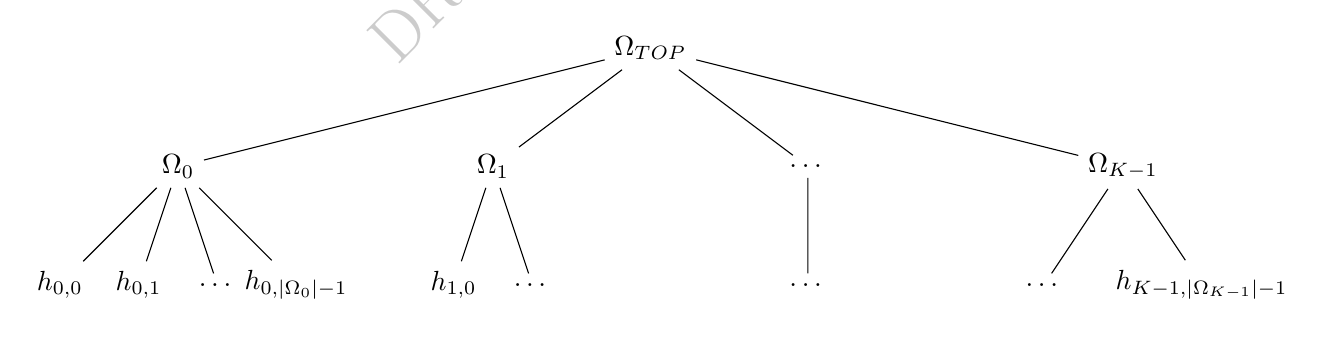
\begin{tikzpicture}
\node {\(\Omega_{TOP}\)} [sibling distance = 4cm]
  child {node {\(\Omega_0\)}  [sibling distance = 1cm]
    child {node {\(h_{0, 0}\)}}
    child {node {\(h_{0, 1}\)}}
    child {node {\dots}}
    child {node {\(h_{0, |\Omega_0| - 1}\)}}
  }
  child {node {\(\Omega_1\)}  [sibling distance = 1cm]
    child {node {\(h_{1, 0}\)}}
    child {node {\dots}}  
  }
  child {node {\dots}
    child {node {\dots}}
  }
  child {node {\(\Omega_{K-1}\)}   [sibling distance = 2cm]
    child {node {\dots}}
    child {node {\(h_{K-1, |\Omega_{K-1}| - 1}\)}}
  };
\end{tikzpicture}

Now let \(\Omega\) be the set of all outcomes \(\Omega_0 \cup \Omega_1 \cup \dots \Omega_{K-1}\), and we create a relative probability function \(P\) with the following assumptions:

1) If the two outcomes fall under the same component, then their relative probabilities do not change:
\[P(h_{k, i}, h_{k, j}) = P_k(h_{k, i}, h_{k, j})\]

2) If the 2 outcomes fall under different components, then their relative probabilities are given as follows:
\[P(h_{k_1, i}, h_{k_2, j}) = P_k(h_{k_1, i}, \Omega_{k_1}) \cdot  P_{TOP}(\Omega_{k_1}, \Omega_{k_2}) \cdot P_{TOP}(\Omega_{k_2}, h_{k_2, j})\]

Theorem: \(P\) respects the fundamental property

Proof: Fill IN

Theorem: \(P\) is totally comparable if and only if the following are true:

1) \(P_{TOP}\) is totally comparable

2) For all \(0 \leq k < K\), \(P_k\) is totally comparable

3) There is at most one component with impossible outcomes with respect to that component. Equivalently, if \(h_{k_1, i}\) and \(h_{k_2, j}\) are two components, and \(P_{k_1}(h_{k_1, i}) = P_{k_2}(h_{k_2, j}) = 0\), then \(k_1 = k_2\). Also equivalently, all components except at most one are totally mutually possible.

Proof: FILL IN

\section{Topology of Relative Probability Spaces}

The idea of a limit distribution requires particularly around the idea of limits. Mathematics can be great at modelling the real world even if it's ideas are theoretically impossible. For example, we might believe that it is impossible for a certain natural process to repeat an infinite number of times, and yet we may still take its value to be infinity in order to get some kind of bound on what that system will look like in the long run. Likewise, it still makes sense to consider a particular outcome in a probabilistic system as certain while maintaining information about the other outcomes in order to calculate the effects of such a limit. [CLEAN UP WORDING OF PARAGRAPH] To this end, we will prove that the space of fully comparable relative distributions is compact.

TODO: Warn people that background in topology is required for this section, and then we can shorten it up! Also, this section can be skipped if not interesting.

One of the benefits of relative probability spaces is their properties with respect to limits. Specifically, if we look at the space of (absolute) categorical distributions on \(\Omega\) and we allow the probability of one outcome to approach 1, then all of the other probabilities will be forced down to 0 and become incomparable with one another. In the relative probability space, the information about the ratios of probabilities of the other outcomes can be preserved even as a single outcome reaches a probability of 1.

If the space of totally comparable RPFs can be shown to be compact, then we know that relative probabilites of outcomes and events are preserved even as they both approach zero relative to another event.

In order to prove compactness, we first must define a topology on the space of totally comparable RPFs. This means identifying the sets that are open (or intuitively, sets that fully surround all of it's members and don't contain its boundary). This starts with finding a \textit{basis of open sets} from which all other open sets can be constructed through countable unions.

For the absolute probability function, we can use \(K-1\)-simplex embedded in \(\mathbb{R}^K\) to get a topology using the standard Euclidean space. There's no obvious way to embed an RPF into euclidean space, so some background is required.

First note that the notion of an open set can change even if a topological space is restricted. For example, on the real number line \(\mathbb{R}\), we take the open interval (0, 1) as an open set (as the term open interval suggests). However, once this is embedded into \(\mathbb{R}^2\), it is now a line segment in a plane and no longer open. It can be thought of as a restriction to an open set on \(\mathbb{R}^2\) to \(\mathbb{R}\). For example, the set \(\{(x, y): x \in (0, 1)\;  \text{and}\;  y \in (-\epsilon, +\epsilon)\}\) given an \(\epsilon > 0\) is such an open set on \(\mathbb{R}^2\). [ILLUSTRATION]

Likewise, an open set on a relative probability space restricted on several outcomes might not be an open set on the relative probability spaces for all of \(\Omega\).

Theorem: Let \(\Omega = \{h_1, h_2\}\) have two elements, with relative probability function \(P\). Then, \(P\) is completely determined by \(P(h_1, h_2)\).

Proof: Let \(q = P(h_1, h_2)\). By the reversed comparison theorem, \(P(h_2, h_1) = q^{-1}\). These values completely determine \(P\) on the event level.

Definition: An \textit{interior open patch} of \(\text{RPF}(\Omega)\) is one of the following:

\begin{enumerate}
  \item If \(K = 2\), a subset parameterized by an interior open interval of magnitudes. \(\{P | a < P(h_1, h_2) < b\}\) for some \(a, b \in \mathbb{M}\) 
  \item If \(K > 2\), a composition of interor patches with composing function \(P_{TOP}\) also being an interior patch.
\end{enumerate}

Intuition: Interior open patches contain only totally mutually possible functions.

Definition: An \textit{exterior open patch} is a one of the following:

\begin{enumerate}
  \item If \(K = 2\), a subset parameterized by an open interval of magnitudes containing 0. \(\{P | 0 \leq P(h_1, h_2) < b\}\) for some \(b \in \mathbb{M}\) 
  \item If \(K > 2\), a composition where \(P_{TOP}\) is an exterior open patch of size 2, and the component that might be zero relative to the other component - \(h_1\) above - is also an exterior open patch while the second component is an interior patch.
\end{enumerate}

Intuition: Exterior open patches contain only totally mutually comparable functions, but some are not totally mutually possible.

TODO: Break this down because it's not that intuitive!

Definition: An \textit{open patch} of \(\text{RPF}(\Omega)\) is a subset of \(\text{RPF}(\Omega)\) that is either an interior or exterior open patch.

Every element of an open patch of \(\text{RPF}(\Omega)\) is totally mutually comparable.

Now let the open patches be the bases for an open set thus defining a topology on the set of totally mutually comparable RPFs of \(\Omega\).

Theorem: The topological space of totally comparable functions on an outcome space \(\Omega\) is \textit{compact}, meaning that for every open cover of it, there is a finite subcover.

Proof:

Let \(K = |\Omega|\). This is going to be an inductive proof where we assume that the theorem is true for all \(k < K\) and then prove that it is true for \(K\).

If \(K \in {0, 1}\) then the set of open sets is finite, so we're good. (Reference degenerate cases)

Let \(h \in \Omega\) be an outcome. The space of totally comparable functions on \(\Omega\) can be split into 2 regions: one where \(P(h, \Omega) = 0\) and one where \(P(h_1, \Omega) > 0\).

- We're going to have to prove this - might be tough!

\subsection{Simple Limit Example}

Let us define a simple relative probability distribution \(P_q\) where \(K = 3\) that is parameterized by the magnitude \(q \in \mathbb{M}\).

Let \(P_q(h_0, h_1) = q\) and \(P_q(h_1, h_2) = 2\).

By the fundamental property, \(P_q(h_0, h_2) :\cong P_q(h_0, h_1) \dot P_q(h_1, h_2) = 2q\).

Now we want to consider the case where the relative probability of \(h_0\) grows infinitely large in comparison to \(h_1\) and \(h_2\).

\[P = lim_{q \rightarrow \infty} P_q\]

We use the following topological definition for the limit in this case: For every open set A of relative probability distributions containing P, there exists an open interval \(B=(b, \infty)\) on \(\mathbb{M}\) such that for every value of \(q \in B\), \(P_q\) is in A.

Proposition: The above limit that defines \(P\) exists, and \(P(h_1, h_2) = 2\). In other words, \(h_2\) is still half as likely as \(h_1\) and that information hasn't been lost on \(P\).

Proof: TODO

\section{Bayesian Inference on Relative Distributions}

A relative probability function represents a belief over the set of potential hypotheses in \(\Omega\).

Start with the traditional Bayesian formula for conditional probability for \(h \in \Omega\) assuming that we recieve data \(D\).

\[P(h|D) = \frac{P(D|h) \cdot P(h)}{P(D)}\]

Now we are going to consider relative probability by looking at the ratio between two hypotheses.

\[\frac{P(h_1|D)}{P(h_2| D)} = \frac{P(D|h_1) \cdot P(h_1)}{P(D)} \div \frac{P(D|h_2) \cdot P(h_2)}{P(D)} = \frac{P(D|h_1) \cdot P(h_1)}{P(D|h_2) \cdot P(h_2)} \]

Next make the following subsitutions:

For the ratio of absolute distributions, subsitute the relative distribution: \(\frac{P(h_1)}{P(h_2} \rightarrow P(h_1, h_2) \)

For the ratio of posterior distributions, subsitute the relative posterior: \(\frac{P(h_1|D)}{P(h_2|D)} \rightarrow P(h_1, h_2|D) \)

The liklihood ratio: \(\frac{P(D|h_1)}{P(D|h_2} \rightarrow P(D|h_1, h_2) \)

Now we get the elegant bayes rule for relative probability:

 \[P(h_1, h_2|D) = L(D|h_1, h_2) P(h_1, h_2)\]
 
 The likelihood ratio \(L(D|h_1, h_2)\) is essentially a description of how the different hypotheses rate the likelihood of data. It is also a relative probability in its own right, and must obey the fundamental properties (cite).
 
 Therefore, the act of bayesian inference is an element-by-element multiplication of two different RPFs \(L(D|h_1, h_2)\) and \(P(h_1, h_2)\). We show that the product of two RPFs obeys the fundamental properties.
 
 Theorem: Let \(P_1\) and \(P_2\) be relative probability functions on \(\Omega\). Define \(P(h_1, h_2) = P_1(h_1, h_2) \cdot P_2(h_1, h_2)\). Then, \(P\) is also an RPF, that it is obeys the fundamental properties.
 
 Proof: Use the multiplication property of the matching relation in equation \ref{eq:matching_multiplication}.
 
 \[P(h_1, h_2)P(h_2, h_3)=P_1(h_1, h_2) P_2(h_1, h_2)P_1(h_2, h_3) P_2(h_2, h_3) :\cong P_1(h_1, h_3) P_2(h_1, h_3)=\]

\[P(h_1, h_1) = P_1(h_1, h_1) P_2(h_1, h_1)=1 \cdot 1=1\]

Theorem: Once two outcome become uncomparable, they will never be comparable again. In other words, if \(P(h_1, h_2)=\ast\), then \(P(h_1, h_2|D) = \ast\).

Proof: \(P(h_1, h_2|D) = L(D|h_1, h_2) P(h_1, h_2) = L(D|h_1, h_2) \cdot \ast = \ast\)

Theorem: Once an outcome becomes impossible with respect to another event, it will either remain impossible or become uncomparable. In other words,  if \(P(h_1, h_2)=0\), then \(P(h_1, h_2|D) \in {0, \ast}\).

Proof: \(P(h_1, h_2|D) = L(D|h_1, h_2) P(h_1, h_2) = L(D|h_1, h_2) \cdot 0\). Normally, this would simplify to 0, but with the matching relation in \(\mathbb{M}^*\), this will be \(\ast\) if \(L(D|h_1, h_2) \in {\infty, \ast}\).

\section{Implementation}

Finally, we implement relative probabiliy as a python class as a demonstration of its usage and relevance.

How to implement this in code, and point to open source example.

Note the connection between magnitude space and the extended real number line, which we can implement through floating point numbers.

This can be implemented by storing K values.

For each category, we have a tier. Items in the same tier are comparable. Each Tier has a parent tier, where items in this teir are said to be impossible relative to anything in its ancestor tiers.

For each category, we also store a floating point number called the value, which should be taken as the log of an unnormalized probability. Note that we will not allow inf or NaN here.

Get the relative probability of 2 categories. Algorithm: If they are in the same tier, then subtract their values and take the exp. If they are in different tiers, do a graph search on the tier. If the first is < the second, the answer is 0. If the first is > the second, the answer is 1. And if they are uncomparable, then the answer is Wildcard, NaN.

Generate and indifferent distribution of category K. Algorithm: Create a single tier where all values are set to 0.

Change the relative probability of item \(k_1\) with respect to \(k_2\), and set it to \(q\). Algorithm: UNSURE

Set the probability \(k_1\) to some absolute value with respect to either the whole distribution, or to its tier.

Randomly sample from this distribution. Algorithm: Only look at the top tier.

Randomly sample from this distribution, but remove certain categories. Algorithm: If the top tier categories are gone, look to see if a top tier remains. If there are multiple top tiers, then there's no way to do it!

Ask: Is this distribution totally mutually possible? Algorithm: Look are a single top tier.

Ask: Is it totally mutually comparable? Algorithm: Look for a linear list of tiers.

\section{Future Work}
\subsection{Expansions to infinite spaces}
- Including topological and metric
- Much richer world, more complex mathematics, more applications
- Is it possible to create a univified version of the Hausdorff measure, where objects are categorized by dimention \(d\), and a smaller-dimentional object is always mutually impossible to a larger dimentional object.
\subsection{Connection Surreal Numbers}
- This is greater, richer than the real number system
- Does this abrograte the need for the relative probability function (not for incomparable values)
- If the infinite case is dealt with above, then more questions are raised about both the power of surreal numbers and their suitability
\subsection{Shrinking the Measure Number System}
- We still have a usable system if we want Rational Numbers
- Can this system work for all non-standard probability value systems?
- There is practical application in this work, since computers cannot work with real numbers directly. We implement this system with floating point numbers and this approximation should be good enough for most applications - but can we have a version with more precise arithmetic

\begin{appendices}

\section{Is an Appendix Needed}

\end{appendices}

%\subsubsection*{References}

\begin{thebibliography}{20}

\bibitem{sklar_dirichlet}Sklar, M. (2014). Fast MLE computation for the Dirichlet multinomial. arXiv preprint arXiv:1405.0099.
\bibitem{sklar_bias}Sklar, M. (2022). Sampling Bias Correction for Supervised Machine Learning: A Bayesian Inference Approach with Practical Applications. arXiv preprint arXiv:2203.06239.
\bibitem{mendelson}Mendelson, B. (1990). Introduction to topology. Courier Corporation.
\bibitem{bradley}Bradley, T. D., Bryson, T., \& Terilla, J. (2020). Topology: A Categorical Approach. MIT Press.
\bibitem{lyon}Lyon, A. (2016). Kolmogorov’s Axiomatisation and its Discontents. The Oxford handbook of probability and philosophy, 155-166.
\bibitem{hajek}Hájek, A. (2003). What conditional probability could not be. Synthese, 137(3), 273-323.

\end{thebibliography}

This document along with revisions is posted at github as https://github.com/maxsklar/relative-probability-finite-paper. See readme for contact information. Local Maximum Labs is an ongoing effort create an disseminate knowledge on intelligent computing.
\end{document}
